\documentclass{article}
\usepackage[utf8]{inputenc}

\usepackage{tikz}
\usetikzlibrary{positioning, fit}

\usepackage{geometry}
\geometry{
top=5mm,
left=5mm,
}

\begin{document}

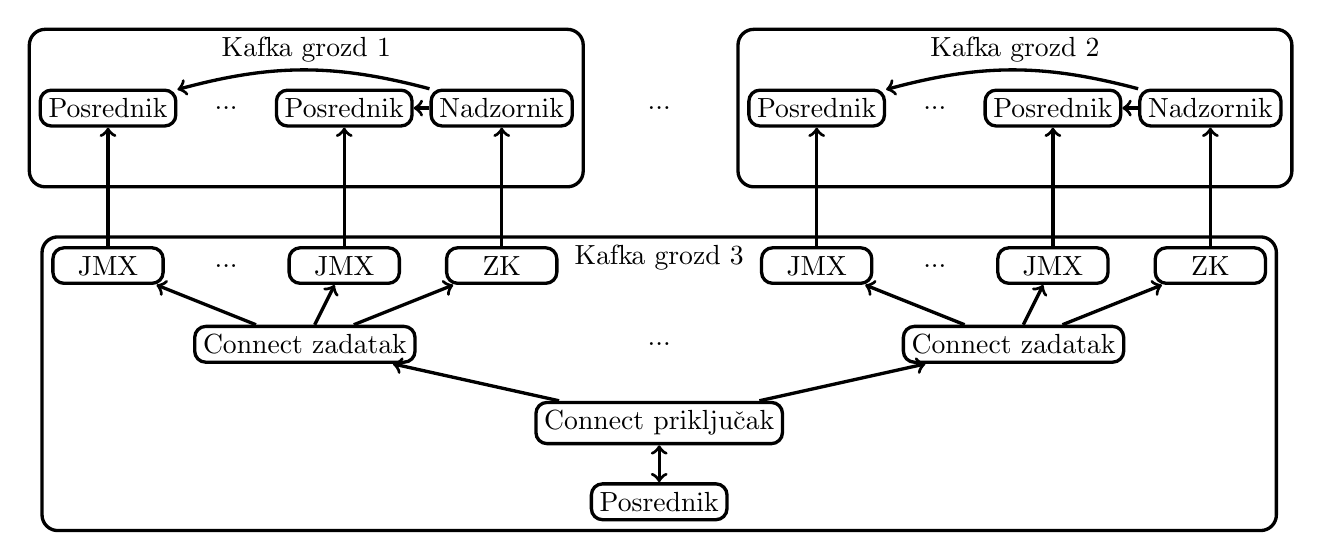
\begin{tikzpicture}[ % has a lot of options; consult the pgf manual
bend angle=15,
long_square/.style={rectangle, draw=black, fill=white, very thick, inner sep=3pt, minimum width=14mm},
rounded_square/.style={rectangle, rounded corners, draw=black, fill=white, very thick, inner sep=3pt, minimum width=14mm},
empty_circle/.style={rectangle, rounded corners=2mm, draw=black, fill=white, very thick, minimum size=4mm},
point/.style={circle, inner sep=0mm},
fit_square/.style={rectangle, rounded corners=2mm, draw=black, very thick, minimum height=20mm},
both_arrow/.style={<->, very thick},
out_arrow/.style={->, very thick},
in_arrow/.style={<-, very thick},
above_edge_text/.style={above, midway, sloped}
]

\node[rounded_square](broker_1) at (0,0) {Posrednik};
\node[](broker_2) at (1.5,0) {...};
\node[rounded_square](broker_3) at (3,0) {Posrednik};
\node[rounded_square](zoo_1) at (5,0) {Nadzornik};

\node[](false_broker) at (7,0) {...};

\node[rounded_square](broker_4) at (9,0) {Posrednik};
\node[](broker_5) at (10.5,0) {...};
\node[rounded_square](broker_6) at (12,0) {Posrednik};
\node[rounded_square](zoo_2) at (14,0) {Nadzornik};

\node[rounded_square](jmx_1) at (0,-2) {JMX};
\node[](jmx_2) at (1.5,-2) {...};
\node[rounded_square](jmx_3) at (3,-2) {JMX};
\node[rounded_square](zk_1) at (5,-2) {ZK};

\node[rounded_square](jmx_4) at (9,-2) {JMX};
\node[](jmx_5) at (10.5,-2) {...};
\node[rounded_square](jmx_6) at (12,-2) {JMX};
\node[rounded_square](zk_2) at (14,-2) {ZK};

\node[rounded_square](task_1) at (2.5,-3) {Connect zadatak};
\node[](task_2) at (7,-3) {...};
\node[rounded_square](task_3) at (11.5,-3) {Connect zadatak};

\node[rounded_square](connector) at (7,-4) {Connect priključak};

\node[rounded_square](kafka) at (7,-5) {Posrednik};

\node[fit_square, fit=(broker_1) (broker_2) (broker_3) (zoo_1)] (cluster_1) {};
\node[anchor=north] at (cluster_1.north) {Kafka grozd 1};

\node[fit_square, fit=(broker_4) (broker_5) (broker_6) (zoo_2)] (cluster_2) {};
\node[anchor=north] at (cluster_2.north) {Kafka grozd 2};

\node[fit_square, fit=(jmx_1) (jmx_2) (jmx_3) (zk_1) (jmx_4) (jmx_5) (jmx_6) (zk_2) (task_1) (task_2) (task_3) (connector) (kafka)] (cluster_3) {};
\node[anchor=north] at (cluster_3.north) {Kafka grozd 3};


\draw[out_arrow](zoo_1) to [bend right] node[auto,swap]{} (broker_1);
\draw[out_arrow](zoo_1) to [] node[auto,swap]{} (broker_3);
\draw[out_arrow](zoo_2) to [bend right] node[auto,swap]{} (broker_4);
\draw[out_arrow](zoo_2) to [] node[auto,swap]{} (broker_6);

\draw[out_arrow](jmx_1) to [] node[auto,swap]{} (broker_1);
\draw[out_arrow](jmx_3) to [] node[auto,swap]{} (broker_3);
\draw[out_arrow](zk_1) to [] node[auto,swap]{} (zoo_1);
\draw[out_arrow](jmx_4) to [] node[auto,swap]{} (broker_4);
\draw[out_arrow](jmx_6) to [] node[auto,swap]{} (broker_6);
\draw[out_arrow](zk_2) to [] node[auto,swap]{} (zoo_2);

\draw[out_arrow](task_1) to [] node[auto,swap]{} (jmx_1);
\draw[out_arrow](task_1) to [] node[auto,swap]{} (jmx_3);
\draw[out_arrow](task_1) to [] node[auto,swap]{} (zk_1);
\draw[out_arrow](task_3) to [] node[auto,swap]{} (jmx_4);
\draw[out_arrow](task_3) to [] node[auto,swap]{} (jmx_6);
\draw[out_arrow](task_3) to [] node[auto,swap]{} (zk_2);

\draw[out_arrow](connector) to [] node[auto,swap]{} (task_1);
\draw[out_arrow](connector) to [] node[auto,swap]{} (task_3);

\draw[both_arrow](kafka) to [] node[auto,swap]{} (connector);

\end{tikzpicture}

\end{document}